
\chapter{Pencarian Akar}

\section{Metode Bagi Dua\label{sec:Bisection}\index{metode bagi dua}\index{metode!bagi dua|see {metode bagi dua}}}

Pada Bagian \ref{sec:Taylor} (halaman \pageref{equationToSolve}),
kita menyatakan bahwa ``$T_{2}(x)$ sebenarnya menghampiri $\ln(x)$
dengan selisih tidak lebih dari $0.1$ pada interval $[3.296,13.13]$'',
seraya berjanji akan membahas perhitungannya nanti. Sekaranglah saatnya.
Pertama-tama, kita nyatakan kembali klaim tersebut sebagai ``jarak
antara $T_{2}(x)$ dan $\ln(x)$ kurang dari atau sama dengan $0.1$
untuk setiap $x\in[3.296,13.13]$.'' Dengan kata lain, 
\[
|T_{2}(x)-\ln(x)|<\frac{1}{10}\quad\mbox{untuk setiap }x\in[3.296,13.13].
\]
Salah satu cara untuk mulai menyelesaikan pertidaksamaan ini adalah
mempertimbangkan pasangan persamaan $T_{2}(x)-\ln(x)=\pm\frac{1}{10}$.
Dengan berfokus pada penyelesaian 
\begin{equation}
T_{2}(x)-\ln(x)=\frac{1}{10},\label{eq:bisectionExample}
\end{equation}
ingat bahwa $T_{2}(x)=2+\frac{x-e^{2}}{e^{2}}-\frac{(x-e^{2})^{2}}{2e^{4}}$.
Jadi, kita hendak menyelesaikan persamaan
\[
2+\frac{x-e^{2}}{e^{2}}-\frac{(x-e^{2})^{2}}{2e^{4}}-\ln(x)=\frac{1}{10}.
\]
Akhirnya, setelah menuliskan persamaan secara lengkap, tidak mengherankan
bahwa kita tidak akan menyelesaikannya untuk $x$ secara eksak. Tidak
ada metode analitik untuk menyelesaikan persamaan semacam itu. Secara
umum, persamaan yang memuat suku polinomial sekaligus suku transendental
tidak dapat diselesaikan secara analitik. Namun, dari grafik pada
Gambar \ref{fig:taylor3}, kita dapat memperoleh hampiran awal bagi
solusinya. Kita mencari titik tempat $T_{2}(x)$ melebihi $\ln(x)$
sebesar $0.1$. Karena kedua grafik hampir berimpit pada $x=6$, kita
dapat menduga bahwa $T_{2}(6)$ melebihi $\ln(x)$ sebesar \textit{kurang
dari} $0.1$ di sana. Karena terdapat celah yang cukup besar antara
kedua grafik pada $x=2$, kita juga dapat menduga bahwa $T_{2}(2)$
melebihi $\ln(x)$ sebesar \textit{lebih dari} $0.1$ di sana. Dengan
kata lain, $T_{2}(2)-\ln(2)>\frac{1}{10}$ sedangkan $T_{2}(6)-\ln(6)<\frac{1}{10}$.
Karena $T_{2}(x)-\ln(x)$ kontinu pada interval $[2,6]$, teorema
nilai antara menjamin adanya nilai $c\in(2,6)$ sedemikian rupa sehingga
$T_{2}(c)-\ln(c)=\frac{1}{10}$. Nilai $c$ inilah yang kita cari.
Kita sudah tahu bahwa nilainya berada di antara 2 dan 6. Ini baru
permulaan, tetapi kita dapat memperoleh hasil yang lebih baik!

Bagaimana dengan 4? Nah, $T_{2}(4)-\ln(4)\approx.04986<0.1$, sehingga
sekarang kita tahu bahwa $T_{2}(4)$ melebihi $\ln(4)$ sebesar \textit{kurang
dari} $0.1$. Sekarang teorema nilai antara memberi tahu kita bahwa
$c$ berada di antara 2 dan 4 ($T_{2}(2)$ melebihi $\ln(x)$ sebesar
\textit{lebih dari} $0.1$). Bagaimana jika kita periksa $x=3$? Mari.
$T_{2}(3)-\ln(3)\approx.131>0.1$, sehingga sekarang kita tahu bahwa
$T_{2}(3)$ melebihi $\ln(3)$ sebesar \textit{lebih dari} $0.1$.
Ringkasnya, $T_{2}(4)-\ln(4)<0.1$ sedangkan $T_{2}(3)\ln(3)>0.1$.
Sekali lagi, berdasarkan teorema nilai antara, kita tahu bahwa $c$
berada di antara 3 dan 4. Kita dapat terus mengulangi proses ini;
batasnya hanyalah kesabaran kita. Proses inilah yang kita sebut \index{metode bagi dua}metode
bagi dua:
\begin{enumerate}
\item Tentukan interval $[a,b]$ sedemikian rupa sehingga salah satu dari
$a$ atau $b$ menghasilkan nilai di atas sasaran, sedangkan yang
lain menghasilkan nilai di bawah sasaran.
\item Hitung titik tengah, $m$, dari interval tersebut.
\item Jika $a$ dan $m$ sama-sama menghasilkan nilai di atas sasaran atau
sama-sama di bawah sasaran, nilai yang dicari terletak dalam $[m,b]$.
\item Jika $b$ dan $m$ sama-sama menghasilkan nilai di atas sasaran atau
sama-sama di bawah sasaran, nilai yang dicari terletak dalam $[a,m]$.
\item Kembali ke langkah 2 dengan menggunakan interval baru tersebut.
\end{enumerate}
\begin{figure}[h]
\caption{\label{fig:bisection-1}$+$ menunjukkan $T_{2}(x)-\ln(x)>\frac{1}{10}$
dan $-$ menunjukkan $T_{2}(x)-\ln(x)<\frac{1}{10}$.}

\centering{}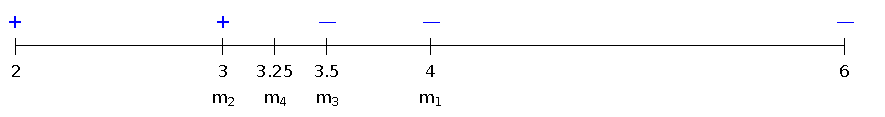
\includegraphics[width=5.5in]{figures/roots-bisection1}
\end{figure}
 Dengan menggunakan tanda $+$ untuk nilai $x$ yang membuat $T_{2}(x)-\ln(x)$
melebihi nilai sasaran $\frac{1}{10}$ dan tanda $-$ untuk nilai
$x$ yang membuat $T_{2}(x)-\ln(x)$ berada di bawah nilai sasaran
$\frac{1}{10}$, kita dapat menggambarkan prosedur ini, termasuk dua
iterasi berikutnya, seperti pada Gambar \ref{fig:bisection-1}. Kita
juga dapat menyajikan kembali perhitungannya dalam sebuah tabel:
\begin{center}
\begin{tabular}{cccccc}
$a$ & $m$ & $b$ & $T_{2}(a)-\ln(a)$ & $T_{2}(m)-\ln(m)$ & $T_{2}(b)-\ln(b)$\tabularnewline
\hline 
2 & 4 & 6 & $.3116$ & $.04986$ & $.002582$\tabularnewline
2 & 3 & 4 & $.3116$ & $0.131$ & $.04986$\tabularnewline
3 & $3.5$ & 4 & $0.131$ & $0.0824$ & $.04986$\tabularnewline
3 & $3.25$ & $3.5$ &  &  & \tabularnewline
\end{tabular}
\par\end{center}

\noindent Bagaimanapun cara kita memahami prosedur tersebut, prosedur
itu menghasilkan barisan hampiran 
\[
4,\ 3,\ 3.5,\ 3.25,\ \ldots
\]
. Berapakah nilai berikutnya? Jawaban \vpageref{subsec:bisectionAnswer1}.

Kita tidak hanya memperoleh barisan bilangan yang mendekati solusi,
tetapi juga mengetahui dengan pasti bahwa $4$ berjarak tidak lebih
dari 2 satuan dari nilai eksak. $3$ berjarak tidak lebih dari 1 satuan.
$3.5$ berjarak tidak lebih dari $0.5$ satuan. Dan $3.25$ berjarak
tidak lebih dari $0.25$ satuan. Secara umum, setiap hampiran berjarak
paling jauh setengah panjang interval tempat hampiran itu dihitung
sebagai titik tengah. Bagaimanapun, nilai eksak dijamin terletak di
dalam interval tersebut. Jarak terjauh yang mungkin antara titik tengah
dan nilai eksak adalah setengah panjang interval.

Walaupun metode ini bekerja dengan baik sebagaimana dijelaskan, biasanya
persamaan yang hendak diselesaikan disederhanakan sehingga salah satu
ruasnya bernilai nol. Dengan demikian, ruas yang lain dapat dipandang
sebagai fungsi yang akarnya dicari. Selain itu, cara ini sedikit menyederhanakan
implementasi metode. Sebagai contoh, kita akan menyelesaikan persamaan
\[
T_{2}(x)-\ln(x)-\frac{1}{10}=0
\]
bukan persamaan \ref{eq:bisectionExample}. Prosedurnya kemudian cukup
berupa pencarian akar fungsi $f(x)=T_{2}(x)-\ln(x)-\frac{1}{10}$.
Karena itulah metode ini disebut metode pencarian akar. Metode ini
digunakan untuk mencari nol, atau akar, suatu fungsi. Dari sudut pandang
ini, delapan iterasi pertama prosedur tersebut dapat diringkas sebagai
berikut:

\begin{center}
\begin{tabular}{cccccc}
$a$ & $m$ & $b$ & $f(a)$ & $f(m)$ & $f(b)$\tabularnewline
\hline 
2 & 4 & 6 & $>0$ & $<0$ & $<0$\tabularnewline
2 & 3 & 4 & $>0$ & $>0$ & $<0$\tabularnewline
3 & $3.5$ & 4 & $>0$ & $<0$ & $<0$\tabularnewline
3 & $3.25$ & $3.5$ & $>0$ & $>0$ & $<0$\tabularnewline
$3.25$ & $3.375$ & $3.5$ & $>0$ & $<0$ & $<0$\tabularnewline
$3.25$ & $3.3125$ & $3.375$ & $>0$ & $<0$ & $<0$\tabularnewline
$3.25$ & $3.28125$ & $3.3125$ & $>0$ & $>0$ & $<0$\tabularnewline
$3.28125$ & $3.296875$ & $3.3125$ &  &  & \tabularnewline
\end{tabular}
\par\end{center}

\noindent Perhatikan dua hal. Nilai sebenarnya dari $f(a)$, $f(m)$,
dan $f(b)$ tidak diperlukan. Hanya tandanya yang penting, sebab kita
hanya perlu mempertahankan satu titik ujung tempat fungsi bernilai
lebih besar daripada 0 (di atas sasaran) dan satu titik ujung tempat
fungsi bernilai kurang daripada 0 (di bawah sasaran). Selain itu,
kolom $f(a)$ dan $f(b)$ sebenarnya juga tidak mutlak diperlukan.
Jika prosedur dijalankan dengan benar, tandanya tidak akan pernah
berubah. Bahkan, itulah arti menjalankan prosedur dengan benar! Pada
langkah 3 dan 4, kita memilih subselang yang dipertahankan dengan
menjaga agar nilai fungsi pada kedua titik ujung berlainan tanda. 

Seperti ditunjukkan oleh baris terakhir, nilai yang dicari kira-kira
$3.296$ sesuai yang dijanjikan. Nilai lainnya, $13.13$, ditentukan
dengan mencari akar fungsi $g(x)=T_{2}(x)-\ln(x)+\frac{1}{10}$. Cobalah!
Misalnya, mulailah dengan $a=10$ dan $b=14$. Penyelesaian \vpageref{subsec:bisectionAnswer2}.

Walaupun berhasil, satu-satunya tujuan nyata menjalankan prosedur
ini menggunakan tabel adalah memastikan bahwa Anda memahami persis
cara kerjanya. Jika benar-benar menggunakan metode ini dalam praktik,
kita akan menulis program komputer singkat sebagai gantinya. Komputer
sangat baik dalam melakukan perhitungan berulang-ulang, sesuatu yang
tidak terlalu dikuasai manusia. Dalam prosedur ini, kita perlu menghitung
titik tengah, memutuskan apakah titik tengah tersebut harus menjadi
titik ujung kiri atau kanan, menetapkannya demikian, lalu mengulanginya. 

Tersisa satu pertanyaan---berapa kali pengulangan, atau iterasi,
perlu kita lakukan? Jawabannya bergantung pada pengguna. Mungkin jawaban
yang berjarak tidak lebih dari $10^{-2}$ dari nilai eksak sudah memadai,
atau mungkin hanya akurasi $10^{-6}$ yang dapat diterima. Program
yang kita tulis harus cukup fleksibel untuk menghitung jawaban dengan
akurasi apa pun yang diinginkan, selama masih dalam batas yang wajar.
Dengan pertimbangan tersebut, berikut kode semu untuk metode bagi
dua. 

\subsection{Analisis Metode Bagi Dua\index{metode bagi dua!analisis}}

Ada dua alasan kuat untuk mempelajari metode bagi dua. Pertama, asumsi-asumsi
yang menjamin keberhasilannya jauh lebih mudah diperiksa daripada
asumsi metode-metode lain. Meskipun demikian, tetaplah berhati-hati.
Pelaksanaan metode numerik apa pun yang benar mensyaratkan pemrograman
yang benar, komputasi yang akurat, dan masukan yang tepat. Pemrogram
dan pengguna dapat berbuat salah. Komputer pun dapat keliru. Ingat
pelajaran dari Bagian \ref{sec:Accuracy}. Sembari bersikap waspada
terhadap hasilnya, imbangi keraguan Anda dengan kepercayaan yang cukup
besar pada metode ini. Hanya dalam keadaan langka komputerlah yang
menjadi sumber masalah.

Kedua, analisis galatnya sederhana. Misalkan $m_{1}=\frac{a+b}{2}$,
yaitu titik tengah $[a,b]$. Misalkan titik-titik tengah berikutnya
adalah $m_{2},\ m_{3},\ m_{4},$ dan seterusnya. Teorema nilai antara
kemudian menjamin $|m_{j}-p|\leq\frac{b-a}{2^{j}}$ untuk suatu akar
$p$ dari $f(x)$. Seperti yang kita pelajari pada Bagian \ref{sec:Speed},
ini berarti barisan $\langle m_{n}\rangle$ berkonvergensi ke $p$
dengan orde linear dan laju kekonvergenan $O\left(\frac{1}{2^{n}}\right)$.
Metode ini patut dianggap lambat berkonvergensi karena ordanya linear.
Namun, di antara metode-metode berorde linear, metode ini patut dianggap
cepat. Galatnya meluruh secara eksponensial---lebih cepat daripada
peluruhan polinomial apa pun.


\subsection{Metode Bagi Dua (Kode Semu)\index{metode bagi dua!kode semu}}

Walaupun secara teknis tidak diperlukan untuk menulis kode, bila memungkinkan
kita akan mengawali kode semu setiap metode dengan asumsi-asumsi matematis
yang menjamin keberhasilannya. Implikasinya adalah bahwa jika metode
dijalankan dalam keadaan ketika asumsi-asumsi tersebut tidak terpenuhi,
metode itu tidak boleh diharapkan memberikan hasil yang dapat diandalkan.
Metode tersebut bisa saja memberikan informasi yang berguna, bisa
juga tidak. Pepatah lama ``sampah masuk...sampah keluar'' berlaku!

\begin{pseudocode} 
\begin{description}
\item [{Asumsi:}] $f$ kontinu pada $[a,b]$. $f(a)$ dan $f(b)$ berlainan
tanda.
\item [{Masukan:}] Interval $[a,b]$; fungsi $f$; akurasi yang diinginkan
$tol$.
\item [{Langkah~1:}] Tetapkan $N=\left\lceil \frac{\ln(b-a)-\ln(tol)}{\ln2}\right\rceil $;
$L=f(a)$;
\item [{Langkah~2:}] Untuk $j=1\ldots N$ lakukan Langkah 3-5:

\begin{description}
\item [{Langkah~3:}] Tetapkan $m=\frac{a+b}{2}$; $M=f(m)$;
\item [{Langkah~4:}] Jika $M=0$ kembalikan $m$;
\item [{Langkah~5:}] Jika $LM<0$ tetapkan $b=m$; jika tidak, tetapkan
$a=m$ dan $L=M$;
\end{description}
\item [{Keluaran:}] Hampiran $m$ yang berjarak tidak lebih dari $tol$
dari akar eksak.
\end{description}
\end{pseudocode}  

Seperti telah disebutkan, metode ini harus menghitung titik tengah
(Langkah 3), memutuskan apakah titik tengah tersebut selanjutnya harus
menjadi titik ujung kiri atau kanan (Langkah 5), menetapkannya sesuai
keputusan itu (Langkah 5), lalu mengulangi proses tersebut beberapa
kali (Langkah 1, 2, dan 4). Sebagian besar kode digunakan untuk menentukan
kapan harus berhenti. Hal ini lazim dalam metode numerik. Perhitungan
adalah separuh tantangan. Mengendalikan perhitungan adalah separuh
lainnya. Jika kita tidak perlu memikirkan penghentian, kode semunya
mungkin tampak seperti ini: 

\begin{pseudocode} 
\begin{description}
\item [{Langkah~1:}] Tetapkan $L=f(a)$;
\item [{Langkah~2:}] Tetapkan $m=\frac{a+b}{2}$; $M=f(m)$; 
\item [{Langkah~3:}] Jika $LM<0$ tetapkan $b=m$; jika tidak, tetapkan
$a=m$ dan $L=M$;
\item [{Langkah~4:}] Kembali ke Langkah 2.
\end{description}
\end{pseudocode}  

\noindent Tidak diperlukan $j$, $tol$, atau $N$, sehingga algoritmanya
menjadi jauh lebih sederhana. Tentu saja, jika diprogram dengan cara
ini, program tidak akan pernah berhenti; karena itu $j$, $tol$,
dan $N$, memang diperlukan. Meskipun demikian, kode semu tanpa kemampuan
untuk berhenti ini penting. Kode tersebut dapat dianggap sebagai inti
program. Inilah kode yang menjalankan metode. Kadang-kadang paling
mudah memulai dari bagian inti, lalu menambahkan kendalinya. 

Mengenai penentuan apakah titik tengah harus menjadi titik ujung kiri
atau kanan, Langkah 5 (Langkah 3 pada inti program) menggunakan cara
yang cukup cerdik. Yang saya maksud dengan cerdik ialah singkat, efisien,
dan tidak langsung tampak jelas. Tanda $LM=f(a)\cdot f(m)$ diperiksa.
Jika nilainya negatif ($LM<0$) maka $m$ harus menjadi titik ujung
kanan (menggantikan $b$) karena ini berarti $f(a)$ dan $f(m)$ berlainan
tanda. Hanya dengan cara itulah $LM$ dapat bernilai negatif. Sebaliknya,
jika $LM>0$ maka kita tahu bahwa $f(a)$ dan $f(m)$ bertanda sama,
sehingga $m$ harus menjadi titik ujung kiri (menggantikan $a$).
Pada Langkah 3, titik tengah dihitung tanpa penjelasan khusus.

Bagian kode lainnya memastikan bahwa program tidak melakukan pekerjaan
melebihi yang diperlukan dan tidak terus mengulang tanpa kemajuan.
Penting untuk dapat memisahkan, setidaknya dalam pikiran Anda, inti
program dari logika penghentian. Mengenai logika penghentian, pada
Langkah 4 kita berhenti jika $err\leq tol$ sebagaimana seharusnya.
Namun, kita juga memeriksa kemungkinan kecil bahwa $M=0$; dalam hal
itu kita kebetulan tepat mengenai akar sehingga harus berhenti.

\subsection*{Konsep Utama}
\begin{description}
\item [{Teorema~Nilai~Antara~menyatakan:}] \index{teorema!nilai antara}Misalkan
$f$ adalah fungsi kontinu pada $[a,b]$ dan $y$ terletak di antara
$f(a)$ dan $f(b)$. Maka terdapat bilangan $c$ di antara $a$ dan
$b$ sedemikian rupa sehingga $f(c)=y$.\footnote{Kata ``di antara'' dalam teorema ini dapat ditafsirkan mencakup
atau tidak mencakup nilai-nilai titik ujung, asalkan penafsiran yang
sama digunakan pada setiap kemunculan kata tersebut.}
\item [{Iterasi:}] (1) Pengulangan suatu perhitungan atau proses lain dengan
menggunakan keluaran satu perhitungan sebagai masukan bagi perhitungan
berikutnya.
\item [{Iterasi:}] (2) Setiap hasil antara dari sebuah iterasi. Disebut
juga hasil iterasi.
\item [{Metode~bagi~dua:}] Menghasilkan barisan hampiran $\langle m_{j}\rangle$
yang berkonvergensi ke suatu akar dalam $[a,b]$.
\item [{Batas~galat~untuk~metode~bagi~dua:}] Galat hampiran $m_{j}$
tidak lebih dari $\frac{b-a}{2^{j}}$. Artinya, $|m_{j}-p|\leq\frac{b-a}{2^{j}}$
untuk suatu akar $p$ dari $f(x)$.
\item [{Kekonvergenan~untuk~metode~bagi~dua:}] Metode bagi dua berkonvergensi
dengan orde linear dan memiliki laju kekonvergenan $O\left(\frac{1}{2^{n}}\right)$.
\end{description}

\subsection*{Octave}

Sekitar separuh upaya untuk menulis kode semu metode bagi dua dikhususkan
pada logika metode---penentuan kapan harus berhenti. Dalam pemrograman,
jenis logika ini ditangani oleh pernyataan \texttt{if then {[}else{]}}\index{Octave!if then [else]@\texttt{if then {[}else{]}}}
beserta variasinya. Dalam pemrograman, tanda kurung siku lazim digunakan
untuk menunjukkan sesuatu yang bersifat opsional. Jadi, pola \texttt{if
then {[}else{]}} harus dibaca sebagai pernyataan bahwa logika ditangani
oleh pernyataan \texttt{if then} atau pernyataan \texttt{if then else}.
Sintaks tepatnya sebagai berikut: \begin{verbatim}
if (condition)
  execute code here
[else
  execute code here]
end%if
\end{verbatim}Sekali lagi, tanda kurung siku menunjukkan kode yang bersifat opsional. 

Pernyataan \texttt{if then} bekerja seperti yang mungkin Anda bayangkan.
Dalam bentuk pernyataan \texttt{if then}, semua kode di antara \texttt{then}
dan \texttt{end} dijalankan setiap kali \texttt{condition} bernilai
benar. Kode tersebut dilewati setiap kali \texttt{condition} bernilai
salah. Bentuk pernyataan \texttt{if then else} serupa. Semua kode
di antara \texttt{then} dan \texttt{else} dijalankan setiap kali \texttt{condition}
bernilai benar. Dalam keadaan ini, kode di antara \texttt{else} dan
\texttt{end} dilewati. Hal yang persis sebaliknya terjadi ketika \texttt{condition}
bernilai salah. Kode di antara \texttt{then} dan \texttt{else} dilewati,
sedangkan kode di antara \texttt{else} dan \texttt{end} dijalankan.
Penggunaan paling sederhana dari pernyataan \texttt{if then else}
mungkin tampak seperti ini. \begin{verbatim}
if (n>10)
  disp('n is big')
else
  disp('n is small')
end%if
\end{verbatim}

\noindent Di Octave, pernyataan \texttt{if then {[}else{]}} ditulis
hampir persis seperti dalam kode semu. Bahkan, sebagian besar kode
semu dalam buku ini dapat diterjemahkan ke Octave hampir kata demi
kata. Satu pengecualian penting adalah simbol yang digunakan dalam
\texttt{condition}. Octave memerlukan operator Boolean dalam kondisi.
Artinya, operator tersebut harus menghasilkan nilai benar atau salah.
Operator \texttt{=} menetapkan suatu nilai kepada variabel. Operator
tersebut bukan operator Boolean sehingga tidak boleh digunakan dalam
kondisi \texttt{if}. Sebagai gantinya, gunakan \texttt{==} (dua tanda
sama dengan). Tabel ini merangkum enam operator Boolean yang paling
umum di Octave.\index{Octave!operator Boolean} \index{Octave!perbandingan}

\begin{center}
\begin{tabular}{c|c}
Perbandingan & Operator\tabularnewline
\hline 
lebih besar dari, lebih kecil dari & \texttt{>}, \texttt{<}\tabularnewline
lebih besar dari atau sama dengan, lebih kecil dari atau sama dengan & \texttt{>=}, \texttt{<=}\tabularnewline
sama dengan & \texttt{==}\tabularnewline
tidak sama dengan & \texttt{!=}\tabularnewline
\end{tabular}
\par\end{center}

\noindent Jika perlu memeriksa apakah $x\geq0$, gunakan \texttt{if
(x>=0)} di Octave. Jika perlu memeriksa apakah $t$ sama dengan 1,
gunakan \texttt{if (t==1)} di Octave. Demikian seterusnya. Operator
logika juga sering diperlukan. 

\begin{center}
\begin{tabular}{c|c}
Operator Logika & Kode Octave\tabularnewline
\hline 
dan & \&\&\tabularnewline
atau & \texttt{||}\tabularnewline
\end{tabular}
\par\end{center}

\noindent Sebagai contoh, jika perlu memeriksa apakah $x$ berada
di antara $a$ dan $b$, seperti pada $a\leq x<b$, diperlukan operator
logika. Dalam hal ini, kita memerlukan ``dan'' logis karena $a\leq x<b$
berarti $a\leq x$ dan $x<b$. Kode Octave-nya adalah \texttt{if (a<=x
\&\& x<b)} atau kode lain yang ekuivalen secara logis.

Secara teknis, pernyataan \texttt{if then} diakhiri dengan pernyataan
\texttt{end}. Namun, untuk menegaskan jenis pernyataan yang diakhiri,
kita akan membiasakan diri mengakhiri pernyataan \texttt{if then}
dengan \texttt{end\%if} dan mengakhiri perulangan \texttt{for} dengan
\texttt{end\%for}. Kode \texttt{\%if} dan \texttt{\%for} hanyalah
komentar karena diawali dengan \texttt{\%}. Oleh karena itu, keduanya
sebenarnya tidak wajib, tetapi dapat membantu keterbacaan kode Anda,
terutama ketika terdapat konstruksi bersarang. Jika terdapat pernyataan
\texttt{if} di dalam perulangan \texttt{for} atau sebaliknya, menggunakan
\texttt{end} untuk mengakhiri keduanya tidak seinformatif menggunakan
\texttt{end\%if} dan \texttt{end\%for}.

Program Octave untuk mencari akar $f(x)=2+\frac{x-e^{2}}{e^{2}}-\frac{(x-e^{2})^{2}}{2e^{4}}-\ln(x)-\frac{1}{10}$
di antara 2 dan 6 dengan galat tidak lebih dari $10^{-4}$ menggunakan
metode bagi dua dapat tampak seperti berikut. \begin{verbatim}
f = @(x) 2+(x-exp(2))/exp(2)-(x-exp(2))^2/(2*exp(4))-log(x)-1/10;
a=2;
b=6;
N=ceil((log(b-a)-log(10^-4))/log(2));
L=f(a);
for i=1:N
  m=(a+b)/2;
  M=f(m);
  if (M==0)
    break;
  end%if
  if (L*M<0)
    b=m;
  else
    a=m;
    L=M;
  end%if
end%for
disp(m);
\end{verbatim} Kode ini menghasilkan jawaban yang benar, \texttt{3.2952}. Bandingkan
kode ini dengan kode semunya. Anda akan melihat bahwa perbedaan utamanya
adalah sintaksis. Namun, menulis kode dengan cara ini memiliki satu
kelemahan besar. Untuk mengubah fungsi, titik-titik ujung, toleransi,
atau jumlah maksimum iterasi, kode harus diubah tepat pada tempatnya.
Hal itu bukan kelemahan nyata jika Anda tidak perlu menjalankan metode
bagi dua lagi. Namun, secara umum, kita seharusnya menganggap bahwa
metode yang kita tulis akan dijalankan berkali-kali dengan masukan
yang berbeda. Atau bahwa kode kita akan diserahkan kepada orang lain
untuk dijalankan berkali-kali dengan masukan yang berbeda. Bayangkan
saya menyerahkan kode ini kepada Anda dan meminta Anda mencari akar
$f(x)=\cos x-x$ di antara 0 dan 3 dengan galat tidak lebih dari $10^{-6}$.
Menanamkan nilai masukan langsung di dalam suatu metode bukanlah praktik
yang baik. Sebaliknya, masukan tersebut harus diberikan sebagai masukan
bagi fungsi yang diprogram. Dalam Octave, hal ini dilakukan dalam
berkas \texttt{.m}. Itu tidak berarti bahwa kita cukup mengambil kode
sebagaimana tertulis dan menyimpannya dalam berkas \texttt{.m}. Berkas
\texttt{.m} akan mengasumsikan bahwa masukan---interval $[a,b]$;
fungsi $f$; dan akurasi yang diinginkan $tol$---akan diberikan
oleh sumber lain, yaitu pengguna. Kode di dalam berkas \texttt{.m}
harus berjalan dengan benar apa pun masukannya yang belum diketahui.
Sintaksis fungsi Octave adalah: \begin{verbatim}
function result=name(input1,input2,...)
  execute these lines
end%function
\end{verbatim} \texttt{function} adalah kata kunci yang memberi tahu Octave bahwa
sebuah fungsi akan didefinisikan. \texttt{result} adalah nama variabel
yang menyimpan jawaban, atau hasil, fungsi tersebut. \texttt{name}
adalah nama fungsi tersebut. Nama ini juga harus menjadi nama berkas
\texttt{.m}. Berkas \texttt{bisection.m} yang lengkap dapat tampak
seperti berikut:\label{bisectionCode} \begin{verbatim}
%%%%%%%%%%%%%%%%%%%%%%%%%%%%%%%%%%%%%%%%%%%%%%%%%%%%%%%%%%%%%%
%  Bisection method written by Leon Q. Brin 09 December 2020 %
%  Purpose: Implementation of the bisection method           %
%  INPUT: Interval [a,b]; function f; tolerance tol.         %
%  OUTPUT: root m to within tol of exact.                    %
%%%%%%%%%%%%%%%%%%%%%%%%%%%%%%%%%%%%%%%%%%%%%%%%%%%%%%%%%%%%%%
function m=bisection(a,b,f,tol)
  N=ceil((log(b-a)-log(tol))/log(2));
  L=f(a);
  for i=1:N
    m=(a+b)/2;
    M=f(m);
    if (M==0)
      return;
    end%if
    if (L*M<0)
      b=m;
    else
      a=m;
      L=M;
    end%if
  end%for
end%function
\end{verbatim} Penulisan seperti ini tidak hanya mudah digunakan kembali; cara ini
juga lebih sederhana! Kita tidak perlu memikirkan fungsi mana yang
akarnya hendak dicari, interval yang digunakan, dan seterusnya. Selain
itu, bentuknya lebih mirip dengan kode semu. Setelah ditulis dan berfungsi
dengan benar, kode tersebut dapat disimpan sebagai berkas \texttt{.m}
dan tidak perlu dilihat lagi, kecuali untuk dipelajari. Kode itu langsung
bekerja! Jika Anda menyerahkannya kepada orang lain untuk digunakan,
orang tersebut semestinya dapat menggunakannya tanpa modifikasi. \texttt{bisection.m}
dapat diunduh dari \href{http://lqbrin.github.io/tea-time-numerical/ancillaries.html}{situs pendamping}.
Sekarang, pencarian akar $f(x)=2+\frac{x-e^{2}}{e^{2}}-\frac{(x-e^{2})^{2}}{2e^{4}}-\ln(x)-\frac{1}{10}$
di antara 2 dan 6 dengan galat tidak lebih dari $10^{-4}$ menggunakan
metode bagi dua dapat dilakukan seperti berikut. \begin{verbatim}
octave:9> 
  f = @(x) 2+(x-exp(2))/exp(2)-(x-exp(2))^2/(2*exp(4))-log(x)-1/10;
octave:10> bisection(2,6,f,10^-4)
ans =  3.2952
\end{verbatim}Setelah \texttt{bisection.m} ditulis, fungsi \texttt{bisection()}
menjadi bagian dari bahasa Octave. Fungsi tersebut dapat dipanggil
sama seperti fungsi bawaan lainnya. Sebagai contoh kedua, kita dapat
mencari akar $f(x)=\cos x-x$ di antara 0 dan 3 seperti berikut: \begin{verbatim}
octave:12> bisection(0,3,@(x) cos(x)-x,10^-5)
ans =  0.7391
\end{verbatim}

\startexercises 

\subsection{Latihan}
\begin{enumerate}
\item \label{exc:bisectionCode}\octave\  Tulislah fungsi Octave yang mengimplementasikan
metode bagi dua seperti ditunjukkan pada \vpageref{bisectionCode}.
Simpan fungsi tersebut sebagai berkas \texttt{.m} untuk digunakan
di kemudian hari.
\item \label{enu:bisectionExamples}Gunakan teorema nilai antara untuk menunjukkan
bahwa fungsi tersebut memiliki akar pada interval yang diberikan.

\begin{enumerate}
\item $f(x)=3-x-\sin x$; $[2,3]$
\item $g(x)=3x^{4}-2x^{3}-3x+2$; $[0,1]$
\item \label{exc:bisection1}$g(x)=3x^{4}-2x^{3}-3x+2$; $[0,0.9]$ \hasasolution 
\item $h(x)=10-\cosh(x)$; $[-3,-2]$
\item \label{enu:failure1}$f(t)=\sqrt{4+5\sin t}-2.5$; $[-6,-5]$
\item \label{enu:failure2}$g(t)=\frac{3t^{2}\tan t}{1-t^{2}}$; $[21.5,22.5]$ \hasasolution 
\item \label{enu:failure3}$h(t)=\ln(3\sin t)-\frac{3t}{5}$; $[1,2]$
\item $f(r)=e^{\sin r}-r$; $[-20,20]$
\item $g(r)=\sin(e^{r})+r$; $[-3,3]$
\item $h(r)=2^{\sin r}-3^{\cos r}$; $[1,3]$
\end{enumerate}
\item \label{exc:bisection2}Buatlah tabel yang menunjukkan tiga iterasi
metode bagi dua dengan fungsi dan interval awal yang diberikan pada
soal \ref{enu:bisectionExamples}. \haspartwithsolution 
\item \label{exc:bisection3}Gunakan kode \texttt{bisection.m} Anda untuk
mencari akar fungsi pada interval dalam soal \ref{enu:bisectionExamples}
dengan galat tidak lebih dari $10^{-8}$. \haspartwithanswer 
\item \label{exc:bisection}Gunakan metode bagi dua untuk mencari $m_{3}$
bagi fungsi yang diberikan pada interval yang diberikan. Kerjakan
tanpa program komputer. Cukup gunakan pensil, kertas, dan kalkulator.
Jika mau, Anda dapat memeriksa jawaban dengan program komputer.  \hasananswer 

\begin{enumerate}
\item $f(x)=\sqrt{x}-\cos x$ pada $[0,1]$
\item $f(x)=3(x+1)(x-\frac{1}{2})(x-1)$ pada $[-1.25,2.5]$
\end{enumerate}
\item \label{enu:useBisection}Gunakan metode bagi dua untuk mencari $m_{4}$
bagi $g(x)=x\sin x+1$ pada $[9,10]$.
\item Gunakan metode bagi dua untuk mencari $m_{3}$ bagi persamaan $x\cos x-\ln x=0$
pada interval $[7,8]$.
\item Gunakan metode bagi dua untuk mencari akar $g(x)=\sin x-x^{2}$ di
antara 0 dan 1 dengan galat mutlak tidak lebih dari $1/4$.
\item Gunakan metode bagi dua untuk menghampiri akar $g(x)=2+x-e^{x}$ di
antara 1 dan 2 hingga galatnya terhadap nilai eksak tidak lebih dari
$0.05$.
\item \label{exc:bisection-2}Terdapat 21 akar fungsi $f(x)=\cos(x)$ pada
interval $[0,65]$. Ke akar manakah metode bagi dua akan berkonvergensi
jika dimulai dengan $a=0$ dan $b=65$? \hasananswer 
\item \label{exc:bisection-1}Tentukan batas jumlah iterasi yang diperlukan
untuk memperoleh hampiran berakurasi $10^{-3}$ bagi solusi $x^{3}+x-4=0$
pada interval $[1,4]$ dengan metode bagi dua. Jangan benar-benar
menghitung hampirannya. Tentukan batasnya saja. \hasasolution 
\item Tentukan batas jumlah iterasi yang diperlukan untuk memperoleh hampiran
berakurasi $10^{-4}$ bagi solusi $x^{3}-x-1=0$ pada interval $[1,2]$
dengan metode bagi dua. Jangan benar-benar menghitung hampirannya.
Tentukan batasnya saja.
\item Grafik $f(x)$ pada interval $[0.75,2]$ ditunjukkan di bawah. Perhatikan
bahwa $f(x)$ memiliki tiga akar pada interval ini, kira-kira $.795$,
$1.06$, dan $1.59$. Jika kita menetapkan $a=.75$ dan $b=2$, ke
akar manakah dari ketiga akar tersebut metode bagi dua berkonvergensi?
Bagaimana Anda mengetahuinya?

\begin{center}
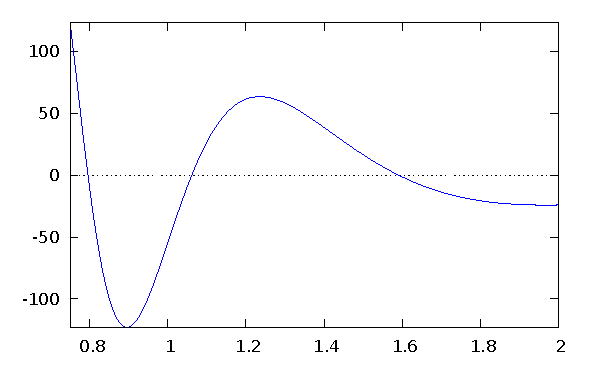
\includegraphics[width=5.5cm]{figures/roots-bisection3}
\par\end{center}
\item Misalkan Anda hendak mencari akar dari $f(x)=x-e^{-x}$ dengan metode
bagi dua. Tentukan sebuah bilangan bulat $a$ sedemikian sehingga
interval $[a,a+2]$ merupakan interval yang sesuai untuk memulai pencarian.
\item Tentukan batas bawah bagi jumlah iterasi yang diperlukan untuk menjamin
akurasi $10^{-20}$ pada soal \ref{enu:useBisection}.
\item \label{exc:bisection-3}Berapa langkah (iterasi) metode bagi dua yang
diperlukan untuk menjamin solusi dengan akurasi $10^{-10}$ jika suatu
akar diketahui berada di dalam $[4.5,5.3]$? \hasananswer 
\item Misalkan Anda menggunakan metode bagi dua pada interval yang panjangnya
3. Berapa iterasi yang diperlukan untuk menjamin bahwa hampiran akurat
hingga $10^{-6}$?
\item Misalkan suatu fungsi $g$ memenuhi asumsi-asumsi metode bagi dua
pada interval yang diberikan. Berawal dari interval tersebut, berapa
iterasi yang diperlukan untuk menghampiri akar dengan toleransi yang
diberikan?

\begin{enumerate}
\item $[-7,10]$; $10^{-6}$
\item $[5,9]$; $10^{-3}$
\item $[9,15]$; $10^{-10}$
\item $[-6,-1]$; $10^{-105}$ (anggaplah komputer menghitung dengan 300
angka signifikan sehingga galat pembulatan tidak menjadi masalah)
\end{enumerate}
\item \octave\ $1$ merupakan akar dari $f(x)=\ln(x^{4}\text{\textminus}x^{3}\text{\textminus}7x^{2}+13x\text{\textminus}5)$
yang tidak dapat dijamin akan ditemukan oleh metode bagi dua. 

\begin{enumerate}
\item Gunakan grafik fungsi di sekitar $1$ untuk menjelaskan mengapa demikian.
Anda dapat menggunakan kode Octave di bawah ini untuk membuat grafik
yang sesuai.
\item Meskipun demikian, jalankan metode bagi dua pada $f$ untuk interval
$[0.8,1.2]$. Apa yang terjadi alih-alih metode tersebut menemukan
akar?
\end{enumerate}
\begin{verbatim}
x=0.8:.01:1.2;
f=@(x) log(x.^4-x.^3-7*x.^2+13*x-5);
plot(x,f(x)) 
\end{verbatim}
\item \octave\ $4$ merupakan akar dari $g(x)=|\sin(\pi x)|$  yang tidak
dapat ditemukan dengan metode bagi dua. 

\begin{enumerate}
\item Gunakan grafik fungsi di sekitar $4$ untuk menjelaskan mengapa demikian.
Anda dapat menggunakan kode Octave di bawah ini untuk membuat grafik
yang sesuai.
\item Meskipun demikian, jalankan metode bagi dua pada $g$ untuk interval
$[3.5,4.5]$. Apa yang terjadi alih-alih metode tersebut menemukan
akar?
\end{enumerate}
\begin{verbatim}
x=3.5:.05:4.5;
f=@(x) abs(sin(pi*x));
plot(x,f(x)) 
\end{verbatim}
\item \label{exc:bisection-4}Misalkan $f(x)=\sin(x^{2})$. $f$ kontinu
pada $[4,5]$, tetapi $f(4)<0$ dan $f(5)<0$, sehingga asumsi-asumsi
metode bagi dua tidak terpenuhi. Meskipun demikian, metode bagi dua
sebagaimana dijelaskan dalam kode semu, jika diterapkan pada $f$
di interval $[4,5]$ \textit{tetap} menghasilkan sebuah akar. Jelaskan. \hasasolution 
\item Fungsi-fungsi pada soal \ref{enu:failure1}, \ref{enu:failure2},
dan \ref{enu:failure3} semuanya tidak memenuhi asumsi-asumsi metode
bagi dua pada interval $[-4,-0.5]$. Untuk setiap fungsi, jelaskan
bagaimana asumsi tersebut gagal terpenuhi.
\item \label{exc:bisection-5}\octave\ Tulislah sebuah fungsi Octave bernama
\texttt{collatz} yang menerima satu masukan bilangan bulat, $n$,
dan mengembalikan $3n+1$ jika $n$ ganjil, serta $n/2$ jika $n$
genap. Simpan fungsi tersebut sebagai berkas \texttt{collatz.m}. Gunakan
pernyataan \texttt{if then else} dalam fungsi Anda. PETUNJUK: Gunakan
fungsi pembulatan ke atas dari Octave. Jika \texttt{ceil(n/2)} sama
dengan \texttt{n/2}, maka \texttt{n} pasti genap (tidak bersisa jika
dibagi 2). Gunakan fungsi \texttt{collatz} Anda untuk menghitung \hasananswer 

\begin{enumerate}
\item \texttt{collatz(17)}
\item \texttt{collatz(10)}
\item \texttt{collatz(109)}
\item \texttt{collatz(344)}
\end{enumerate}
\item \octave\ Tulislah fungsi nilai mutlak Anda sendiri yang bernama \texttt{absval}
(\texttt{abs} sudah didefinisikan oleh Octave, sehingga sebaiknya
Anda menggunakan nama lain), yang menerima masukan bilangan riil dan
mengembalikan nilai mutlak masukan tersebut. Gunakan pernyataan \texttt{if
then else} dalam fungsi Anda. Simpan fungsi tersebut sebagai \texttt{absval.m}
dan ujilah dengan perhitungan berikut. 

\begin{enumerate}
\item $|-3|$
\item $|123.2|$
\item $\left|\pi-\frac{22}{7}\right|$
\item $|10-\pi^{2}|$
\end{enumerate}
\item \label{exc:bisection-6}$f(x)=\sin(x^{2})$ memiliki lima akar pada
interval $[7,8]$. $f(7)<0$, $f(8)>0$, dan $f$ kontinu pada $[7,8]$,
sehingga asumsi-asumsi metode bagi dua terpenuhi. Metode tersebut
akan konvergen ke suatu akar.

\begin{enumerate}
\item Gunakan berkas \texttt{bisection.m} Anda (Latihan \ref{exc:bisectionCode})
untuk menentukan akar mana yang diperoleh. \hasananswer 
\item Temukan 4 interval berbeda yang membuat metode bagi dua konvergen
ke empat akar lainnya di $[7,8]$.
\end{enumerate}
\item Fungsi yang ditampilkan memiliki akar kira-kira di $2.41$, $4.11$,
$5.62$, $7.01$, $8.32$, $9.57$, $10.78$, dan $11.94$. Dengan
interval awal yang diberikan, ke akar mana metode bagi dua akan konvergen?

\begin{center}
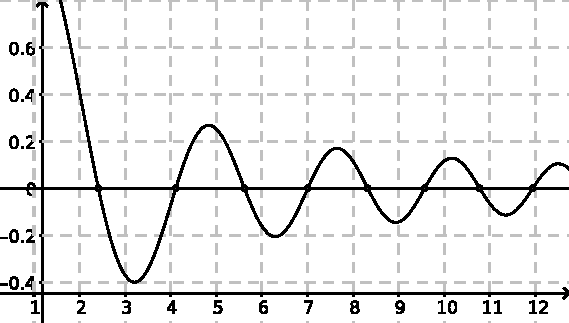
\includegraphics[scale=0.6]{figures/roots-bisection2}
\par\end{center}
\begin{enumerate}
\item $[2,3]$
\item $[6,8]$
\item $[2,6]$
\item $[5,9]$
\item $[10,12]$ Catatan: asumsi metode bagi dua tidak terpenuhi pada interval
ini. Meskipun demikian, metode sebagaimana diuraikan dalam kode semu
\textit{akan} konvergen ke suatu akar!
\end{enumerate}
\item Carilah interval dengan panjang 1 yang memungkinkan metode bagi dua
diterapkan untuk mencari akar dari $f(x)=x^{4}-7.6746x^{3}-40.7477022x^{2}+200.9894434x+319.0914281$.
\item Algoritma berikut merupakan salah satu bentuk metode bagi dua.

\begin{pseudocode} 
\begin{description}
\item [{Asumsi:}] $f$ kontinu pada $[a,b]$. $f(a)$ dan $f(b)$ memiliki
tanda yang berlawanan.
\item [{Masukan:}] Interval $[a,b]$; fungsi $f$
\item [{Langkah~1:}] Untuk $j=1\ldots15$ lakukan Langkah 2 dan 3:

\begin{description}
\item [{Langkah~2:}] Tetapkan $m=\frac{a+b}{2}$;
\item [{Langkah~3:}] Jika $f(a)f(m)<0$ maka tetapkan $b=m$; jika tidak,
tetapkan $a=m$;
\end{description}
\item [{Langkah~4:}] Cetak $m$.
\item [{Keluaran:}] Hampiran $m$.
\end{description}
\end{pseudocode} 
\begin{enumerate}
\item Terapkan algoritma ini pada fungsi $f(x)=(x)(x-2)(x+2)$ pada interval
$[-3,3]$. Akar manakah yang akan dihampiri algoritma ini?
\item Berapakah batas galat yang dijamin bagi hampiran tersebut menurut
rumus
\[
|p_{n}-p|\leq\frac{b-a}{2^{n}}?
\]
\item Seberapa akurat hampiran tersebut sebenarnya? Bandingkan dengan batas
pada (b).
\item Ubahlah algoritma agar dapat menghampiri akar yang berbeda dengan
menggunakan interval awal yang sama.
\item Ubahlah algoritma agar tidak menggunakan perkalian.
\end{enumerate}
\item \label{bisectionCode-1}Gunakan kode semu berikut untuk menulis implementasi
metode bagi dua yang sedikit berbeda. Lihat Tabel \ref{tab:commonOctave}
jika Anda belum yakin cara memprogram besaran $\lceil(\ln(b-a)-\ln(TOL))/\ln2\rceil$.
Perulangan while dibahas pada \vpageref{subsec:WhileLoop}.

\begin{description}
\item [{Masukan:}] fungsi $f$, titik ujung $a$ dan $b$; toleransi $TOL$.
\item [{Kembalikan}] solusi hampiran $p$ beserta nilai $f(p)$ dan jumlah
iterasi yang telah dilakukan $N_{0}$.
\item [{Langkah~1}] Tetapkan $i=1$; $FA=f(a)$; $N_{0}=\lceil(\ln|b-a|-\ln(TOL))/\ln2\rceil$;
\item [{Langkah~2}] Selama $i\leq N_{0}$ lakukan Langkah 3 sampai 6.

\begin{description}
\item [{Langkah~3}] Tetapkan $p=(a+b)/2$; $FP=f(p)$;
\item [{Langkah~4}] Jika $FP=0$ maka\\
$\qquad$Kembalikan($p$, $f(p)$, $i$); BERHENTI.
\item [{Langkah~5}] Tetapkan $i=i+1$;
\item [{Langkah~6}] Jika $FA\cdot FP>0$ maka\\
$\qquad$Tetapkan $a=p$; $FA=FP$;\\
jika tidak\\
$\qquad$Tetapkan $b=p$;
\end{description}
\item [{Langkah~7}] Kembalikan($p$, $f(p)$, $N_{0}$);\\
BERHENTI.
\end{description}
\begin{enumerate}
\item Bahas kelebihan dan kekurangan algoritma ini dibandingkan dengan algoritma
pada \vpageref{bisectionCode}.
\item Dari manakah perhitungan $N_{0}=\lceil(\ln(b-a)-\ln(TOL))/\ln2\rceil$
diperoleh?
\end{enumerate}
\item Gunakan kode yang Anda tulis untuk soal \ref{bisectionCode-1} untuk
mencari solusi dengan galat tidak lebih dari $10^{-5}$ bagi persoalan-persoalan
berikut. 

\begin{enumerate}
\item $x-2^{x}+.95=0$ pada $[0,1]$
\item $e^{x}-x^{2}+3x-2=0$ pada $[0,1]$
\item $2x\cos(2x)-(x+1)^{2}=0$ pada $[-3,-2]$ dan pada $[-1,0]$
\end{enumerate}
\item Carilah hampiran $\sqrt{3}$ dengan galat tidak lebih dari $10^{-4}$
menggunakan metode bagi dua. Tulislah esai tentang cara Anda menyelesaikan
masalah ini. Sertakan kode metode bagi dua Anda, fungsi dan interval
yang Anda gunakan, serta alasan pemilihannya.
\item Sebuah palung sepanjang $L$ memiliki penampang berbentuk setengah
lingkaran berjari-jari $r$. Jika diisi air hingga permukaan air berada
pada jarak $h$ dari bagian atas, volume air $V$ adalah 
\[
V=L\left[0.5\pi r^{2}-r^{2}\arcsin\left(\frac{h}{r}\right)-h\sqrt{r^{2}-h^{2}}\right]
\]
Misalkan $L=10$ kaki, $r=1$ kaki, dan $V=12.4$ kaki$^{3}$. Tentukan
kedalaman air di dalam palung dengan galat tidak lebih dari 0,01 kaki.
Catatan: Di Octave, gunakan \texttt{asin(x)} untuk $\arcsin(x)$ dan
\texttt{pi} untuk $\pi$.
\end{enumerate}
\finishexercises

\subsection*{Jawaban}
\begin{description}
\item [{Berapakah~nilai~yang~diperoleh~berikutnya?}] \label{subsec:bisectionAnswer1}
$T_{2}(3.25)-\ln(3.25)\approx.10429$, yang melebihi nilai sasaran.
Jadi $3.25$ menjadi titik ujung kiri yang baru, dan nilai berikutnya
adalah $\frac{3.25+3.5}{2}=3.375$, yaitu titik tengah dari $3.25$
dan $3.5$.
\item [{Titik~ujung~kanan~adalah~$13.13$:}] \label{subsec:bisectionAnswer2}
Dengan memulai dari $a=10$ dan $b=14$, perhatikan bahwa $g(a)\approx.088>0$
dan $g(b)\approx-.044<0$, sehingga nilai $g$ pada titik ujung kiri
harus selalu positif dan nilai $g$ pada titik ujung kanan harus selalu
negatif:
\end{description}
\begin{center}
\begin{tabular}{ccccc}
$a$ & $m$ & $b$ & $g(m)$ & \tabularnewline
\hline 
10 & 12 & 14 & $.044$ & $\Rightarrow m$ menjadi titik ujung kiri\tabularnewline
12 & 13 & 14 & $.006$ & $\Rightarrow m$ menjadi titik ujung kiri\tabularnewline
13 & $13.5$ & 14 & $-.017$ & $\Rightarrow m$ menjadi titik ujung kanan\tabularnewline
13 & $13.25$ & $13.5$ & $-.005$ & $\Rightarrow m$ menjadi titik ujung kanan\tabularnewline
13 & $13.125$ & $13.25$ & $.0004$ & $\Rightarrow m$ menjadi titik ujung kiri\tabularnewline
$13.125$ & $13.1875$ & $13.25$ & $-.002$ & $\Rightarrow m$ menjadi titik ujung kanan\tabularnewline
$13.125$ & $13.15625$ & $13.1875$ & $-.0009$ & $\Rightarrow m$ menjadi titik ujung kanan\tabularnewline
$13.125$ & $13.140625$ & $13.15625$ & $-.0002$ & $\Rightarrow m$ menjadi titik ujung kanan\tabularnewline
$13.125$ & $13.1328125$ & $13.140625$ &  & \tabularnewline
\end{tabular}
\par\end{center}
